\section{Data-Structures \& Diagrams}
\begin{figure}[H]
    \centering
    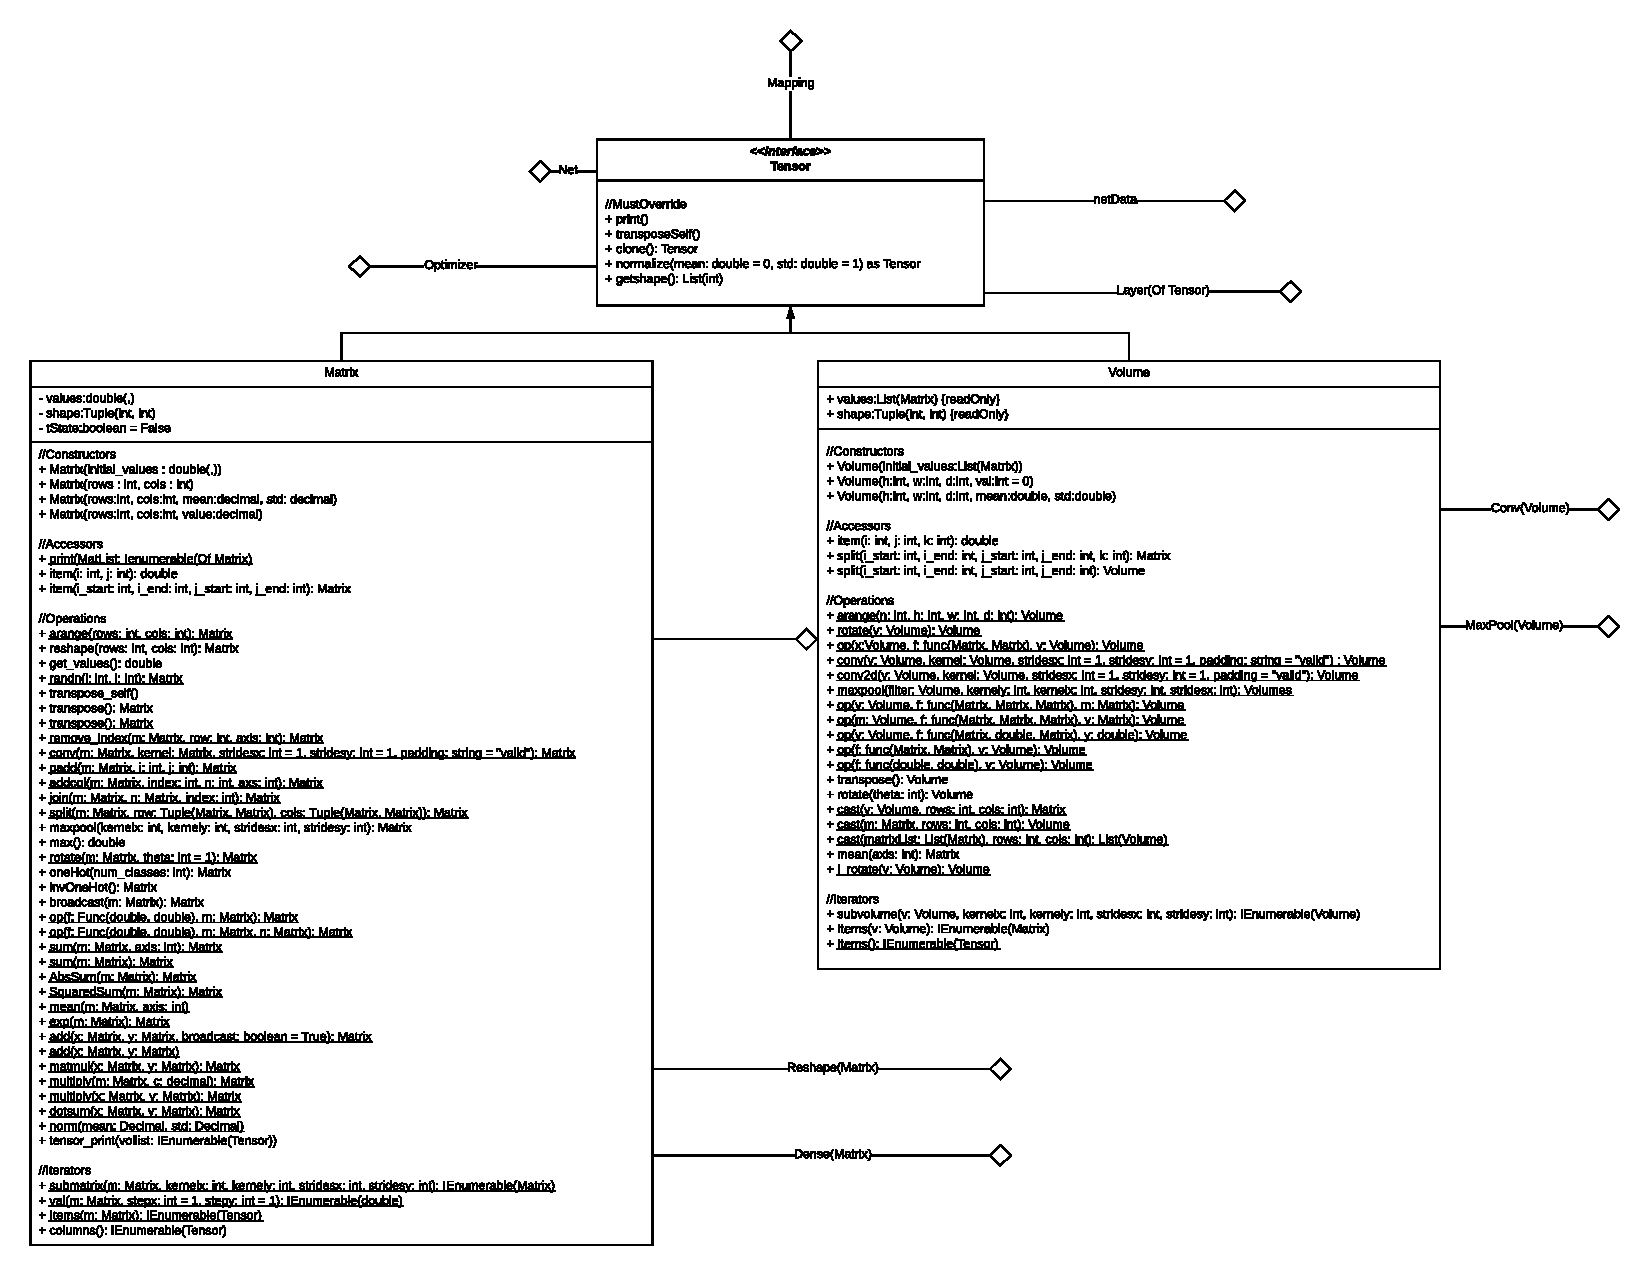
\includegraphics[width=18cm, height=18cm, angle=90]{Design/Overview/UMLCharts/NeuralDotUMLSeperated-Tensor.pdf}
    \caption{Class Diagram for NeuralDot Library - Tensors}
    \label{fig:Class Diagram for NeuralDot Library - Tensors}
\end{figure}

\begin{figure}[H]
    \centering
    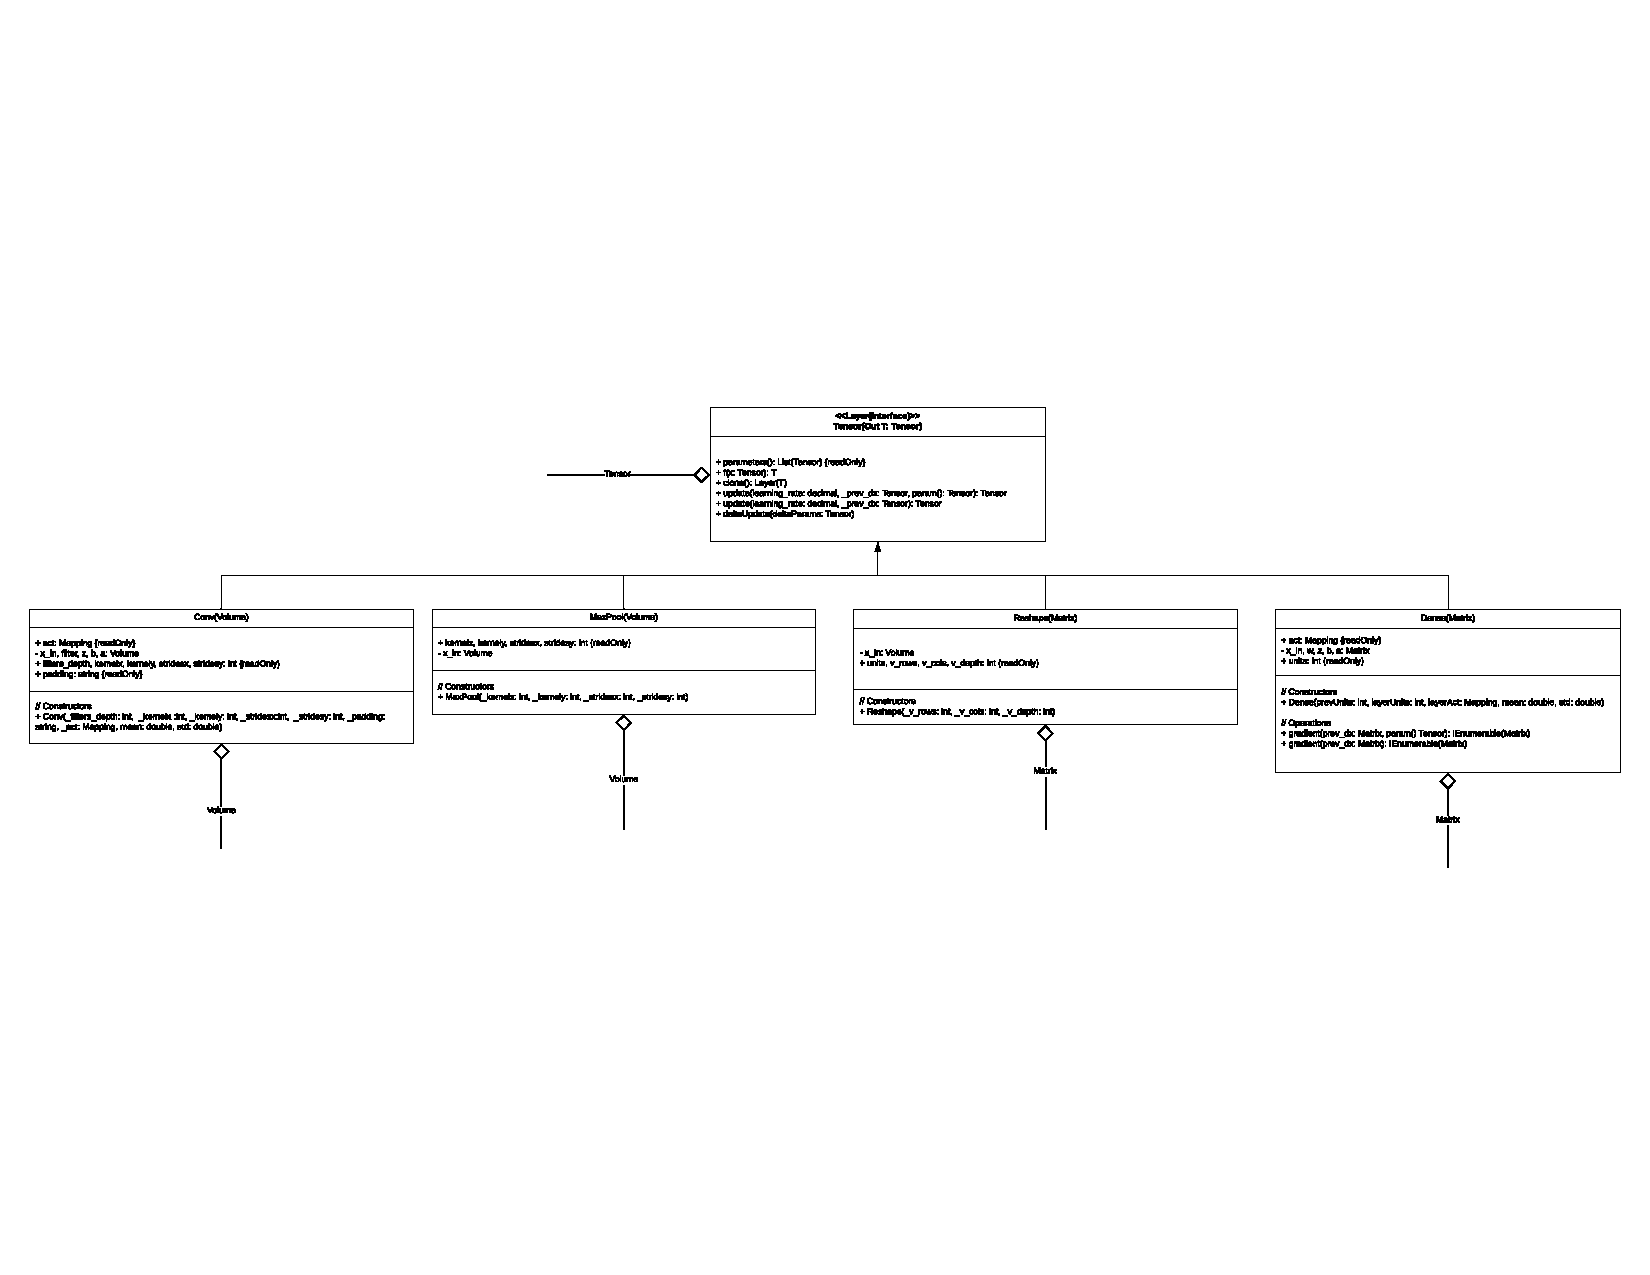
\includegraphics[width=18cm, height=18cm, angle=90]{Design/Overview/UMLCharts/NeuralDotUMLSeperated-Layer.pdf}
    \caption{Class Diagram for NeuralDot Library - Layers}
    \label{fig:Class Diagram for NeuralDot Library - Layers}
\end{figure}

\begin{figure}[H]
    \centering
    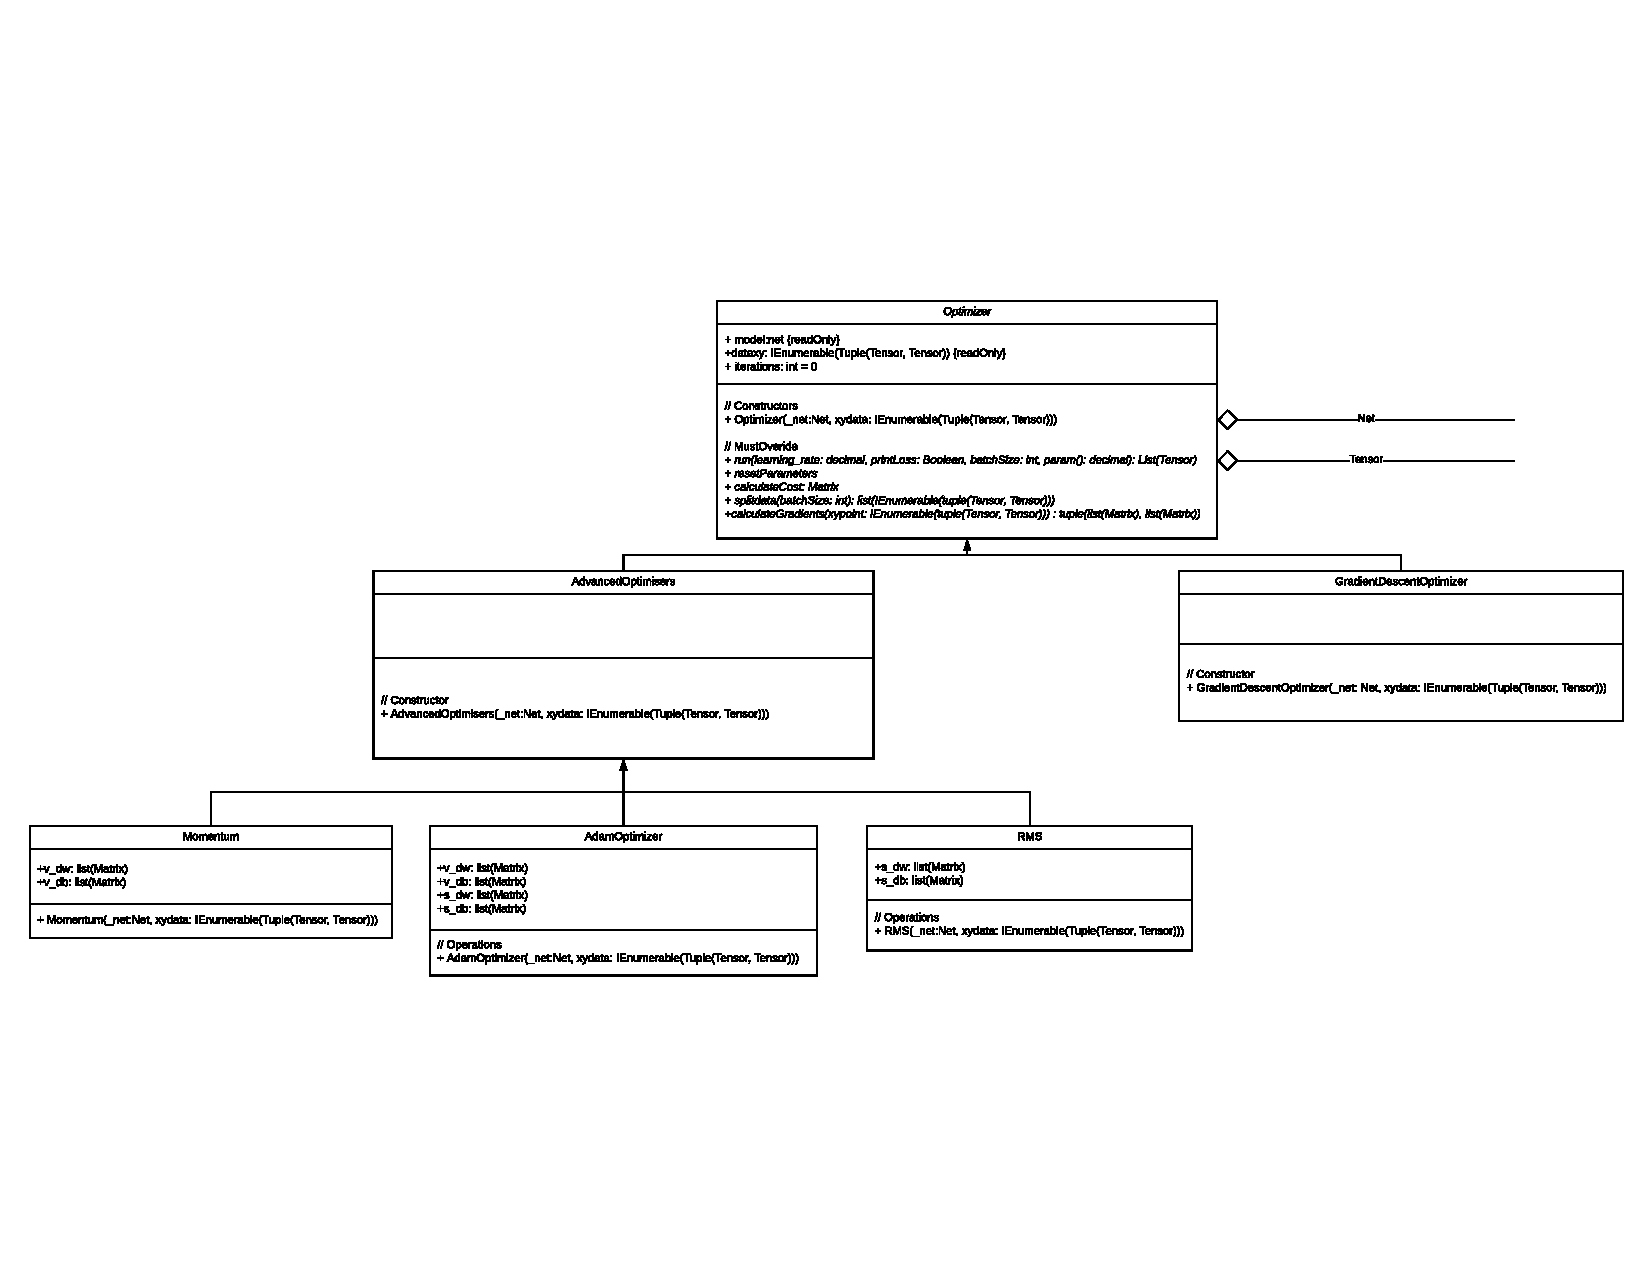
\includegraphics[width=18cm, height=18cm, angle=90]{Design/Overview/UMLCharts/NeuralDotUMLSeperated-Optimisers.pdf}
    \caption{Class Diagram for NeuralDot Library - Optimisers}
    \label{fig:Class Diagram for NeuralDot Library - Optimisers}
\end{figure}

\begin{figure}[H]
    \centering
    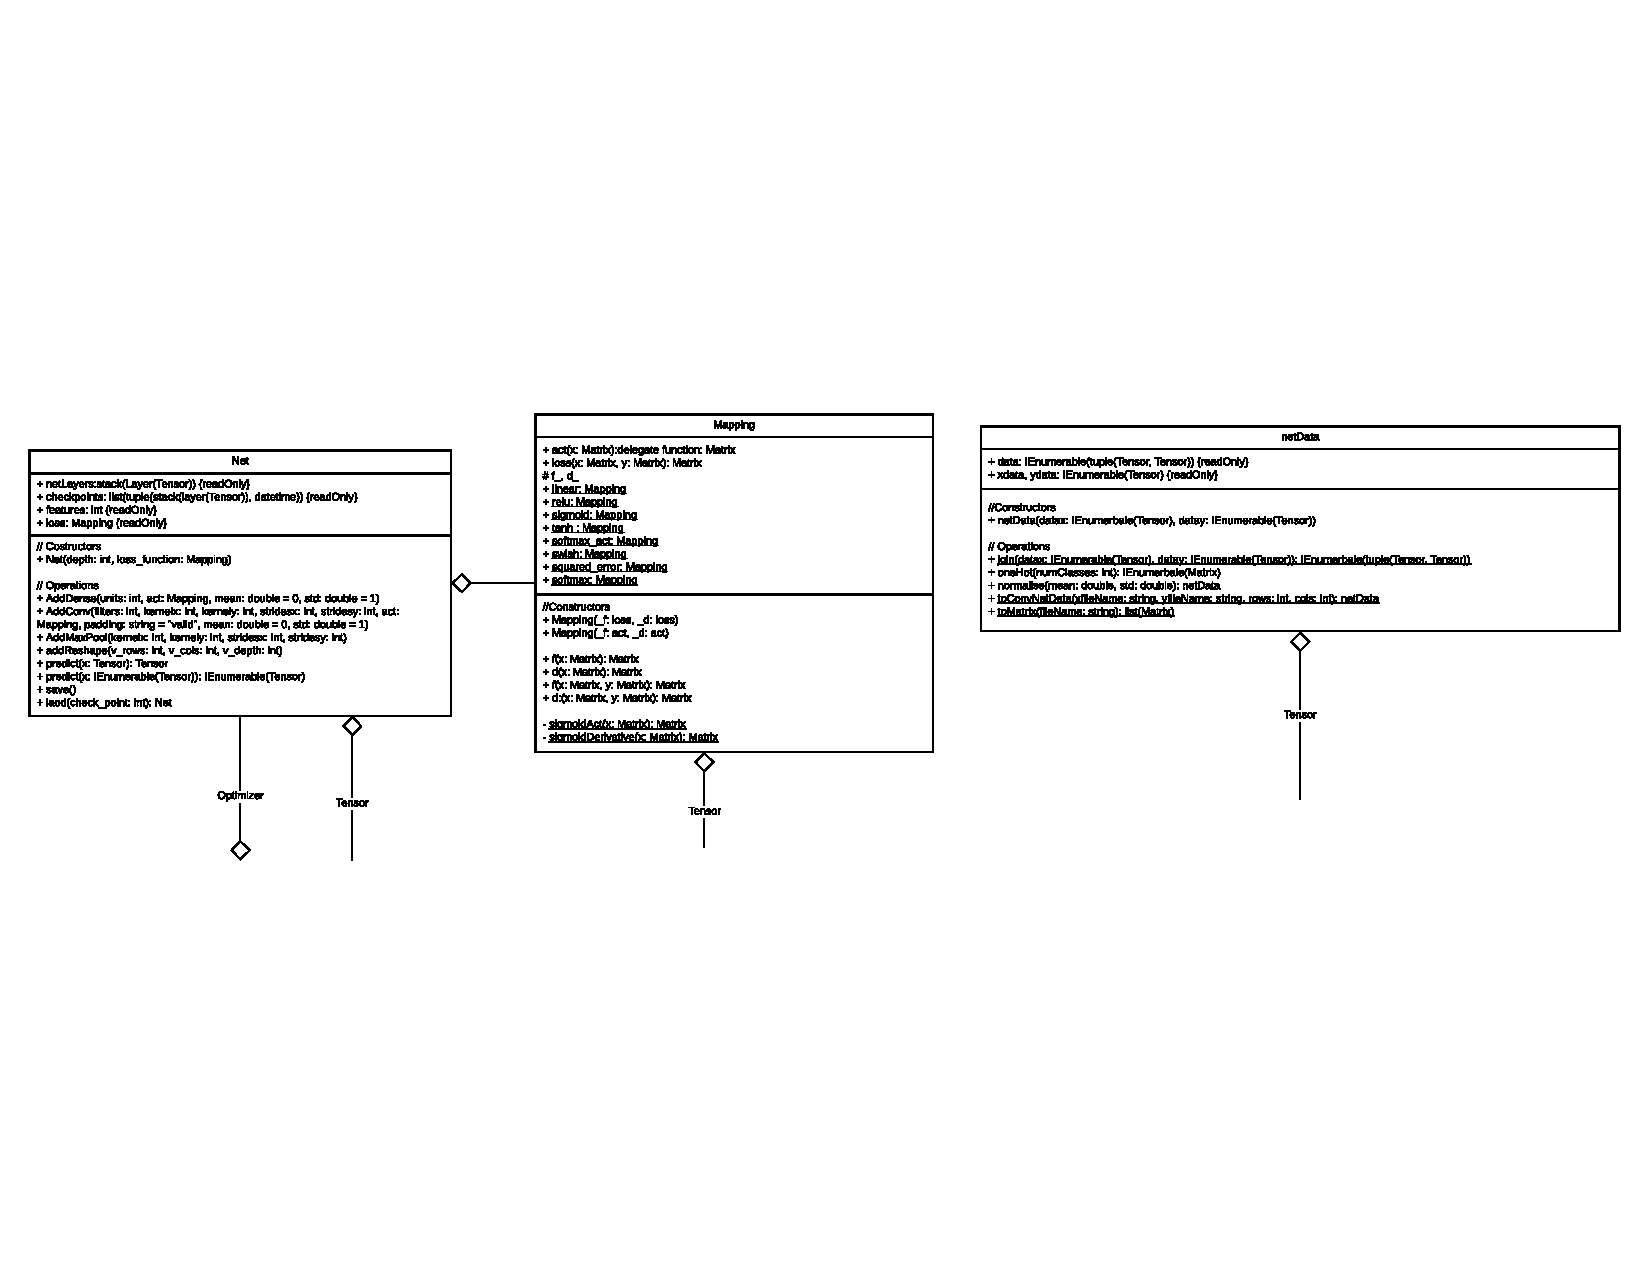
\includegraphics[width=18cm, height=18cm, angle=90]{Design/Overview/UMLCharts/NeuralDotUMLSeperated-Net.pdf}
    \caption{Class Diagram for NeuralDot Library - Net}
    \label{fig:Class Diagram for NeuralDot Library - Net}
\end{figure}

The figures above shows the UML for the NeuralDot library. The class \textbf{Tensor}, is a base class for the class \textbf{Matrix} and \textbf{Volume}, as both classes have functions in common. This base class is also necessary, as the \textbf{layers} class is a \textit{generic base class} of Tensor. Therefore, it is necessary to have \textbf{volume} and \textbf{matrix} \textit{inherit} from \textbf{Tensor}, as some layers will be of type \textbf{Volume}, and some of \textbf{Matrix}. The class \textbf{matrix} includes all the functions, iterators and subroutines that the user may use and the same applies for the \textbf{Volume} Class. In addition to the sub-routines, functions and iterators, I have also added \textit{shared operators} to both classes such as +, -, *, and /. These operators makes using matrices and volumes more accessible and intuitive for beginners making the library more user-friendly to work with.
\\ \\
The \textbf{Layer} class is a \textit{generic interface} of type \textbf{Tensor}. The classes \textbf{Dense}, \textbf{Conv}, \textbf{MaxPool} and \textbf{Reshape} all \textit{extend} from \textbf{Layer}, as they all have the same functions and are all layers. The class \textbf{Layer} includes all the main functionalities required by any specific layer such as updating the layer, retrieving the parameters and so on. Besides the class \textbf{Dense}, every other class that implements Layers, do not have any other functions besides the ones they override from the base class. The class \textbf{Dense}, which implements \textit{layer(Of Matrix)}, has 2 extra functions called gradient each which return the gradient for a particular back-prop iteration given the previous layers gradients, with the only difference being that one of them only works if it is the final layer in the net. These extra functions are there so that the advanced optimisation methods can then be used to train these dense nets, allowing the user to gain an intuition onto which optimisation method works best for which particular architecture or data. Furthermore, these extra functions also allow the user to view the gradients for a particular training iterations, which is something the user asked for in the interview process, therefore I have added these extra functions to the \textbf{Dense} class only as my main focus was on Dense nets.
\\ \\
Finally, the class \textbf{Net} adds functionality to the network enabling users to add layers to their net and choose the loss function being used as well as the activations at each layer. Another functionality, I added to the \textbf{Net} class is that I allowed the user to save models in a list, enabling the user to have many models. This is so that the user can then experiment with different architectures, optimisation techniques and loss functions and then compare the impact each has on the overall outcome on the Net. After saving these models, the user can then load the net back from the list, called checkpoints, and then re-use this loaded Net.
